\documentclass[a4paper,fontsize=11pt,report,notitlepage,line_length=38zw,number_of_lines=40,dvipdfmx]{jlreq}
%\usepackage{xltxtra}
%\usepackage{zxjatype}
%\setjamainfont[BoldFont=ipaexm.ttf]{ipaexm.ttf}
%\setjasansfont[BoldFont=ipaexg.ttf]{ipaexg.ttf}

\usepackage{amsmath}
\usepackage{amssymb}
\usepackage{booktabs}
\usepackage{cite}
\usepackage[dvipdfmx]{graphicx}


\title{日本の中古住宅市場における\\スマートコントラクト活用効果の検証}
\author{
学籍番号:57195017 氏名:高橋 宏輝
\\ゼミ名称:ブロックチェーンと分散ファイナンス演習
\\主査:斉藤 賢爾 教授 副査:中里 大輔 教授}

\begin{document}
\date{}
\maketitle
\begin{abstract}
本稿では、日本の中古住宅市場を対象として、住宅の売買取引においてスマートコントラクトをどのように導入することができるか検討するとともに、スマートコントラクトの活用により住宅の品質や価格の情報が円滑に共有されることで、住宅の取引価格にどのような影響を及ぼすか検証する。
日本の中古住宅市場は売主、買主といった市場参加者の間で住宅の品質などの情報の非対称性が高く、いわゆるレモンの市場であると指摘されている。品質などの情報の非対称性が高い結果、買主は購入する住宅の品質が低い可能性を想定し、低い値付けをする。市場に供給される住宅が全て低く値付けされることで、質の良い住宅が市場に供給されにくい悪循環が起きている。また、住宅の品質向上に必要なリフォームも、品質情報が共有されない市場では取引価格の引き上げ効果が期待できないために実施されず、住宅ストック全体の品質向上を妨げている。このような中古住宅市場の問題により、家計が保有する住宅の資産価値は低くなり、家計の活発な消費や投資に繋がらない。

中古住宅市場における情報の非対称性を解消する手法として、スマートコントラクトを活用した住宅取引の導入を考える。スマートコントラクトはブロックチェーン上で資産の移転などの処理を行うプログラムである。スマートコントラクトによる資産の移転はブロックチェーン上に改ざん出来ない形で記録され、ブロックチェーンの参加者は誰もがこれらの情報を参照することができる。住宅市場へのスマートコントラクトの活用は、契約当事者双方の確実な債務履行や無権利者の取引参加を排除するといったエスクローとしての活用が中心であった。しかし、情報の非対称性が高い住宅市場においては、エスクローとしての活用に加えて、実際の住宅取引の情報を参照できるデータベースとしての活用の価値も大きい。ただし、実際の住宅取引の情報は取引参加者のプライバシーに関わる情報である事から、データベースとしての利用にあったては、参照される情報に一定の匿名性を持たせる必要がある。本稿では、これらの点を考慮したスマートコントラクトの仕様を検討する。スマートコントラクトの活用によって住宅の品質や過去の取引価格などの情報が全ての参加者から参照可能となった場合、住宅の取引価格にどのような影響が発生するかの検証には、住宅取引を単純化したゲームによるマルチエージェントシミュレーションを行った。シミュレーションでは、品質の情報が買主から参照可能になる事によって、市場全体として見た場合の売主の利得は向上し、成約率も改善することが確認できた。

日本の住宅市場では、人口が既に減少に転じており、800万戸を超える住宅が空き家になっているにもかかわらず、年間90万戸の住宅が新たに供給されている。このような状況は、中古住宅市場の情報の非対称性により質の良い中古住宅が市場に供給さず、市場が活性化しないことが影響していると考えられる。スマートコントラクトでの住宅取引により情報の非対称性が解消され、住宅が品質に応じて適正に値付けされる市場を形成できれば、質の良い中古住宅の市場供給も増え、取引量も増えると考えられる。

\end{abstract}

\newpage
\tableofcontents

\newpage
\chapter{序論}
日本の住宅市場は新築住宅に偏重しており、中古住宅の流通量は少ない。2015年の国土交通白書によると日本の住宅取引全体に占める中古住宅取引の割合は14.7\%であり、アメリカ(同89.3\%)、イギリスの(同88.0\%)、フランス(同68.4\%)と比較して大幅に低い水準となっている\cite{hakusho}。一方で、総務省の住宅・土地統計調査によると、日本の住宅総数は、2018年の段階で総世帯数に対して約879万戸超過している。居住者のいない住宅の存在は都市部でも顕著であり、首都圏の一都三県における居住者のいない住宅戸数は200万戸を超えている。しかし、中古住宅市場の流通量は少なく、これらの居住者がいない住宅ストックの活用が進んでいない。このため、日本の住宅は新築から25年程度で建物の価値が半分になると指摘されている(吉田 2016)\cite{yoshida2016}。
また、住宅が平均して建築後何年で取り壊されているかを調査した滅失住宅の平均築後年数は、日本が32.1年に対してアメリカは66.6年、イギリスは80.6年となっている\cite{kizonjutaku}。

諸外国よりも相対的に短い期間で建物の価値が減少する傾向にあるものの、住宅は日本の家計の資産構成において大きな割合を占めている。日本の家計が保有する住宅・宅地資産の総額は1,000兆円を超えると言われており、家計が保有する現金・預金等の総額940兆円を上回る。しかし、日本において住宅の建物部分の価値は短い期間で減少してしまうため、国内でこれまでに行われた住宅投資の累計が約890兆円にのぼるのに対し、その現在評価額は投資額累計を500兆円以上下回る約350兆円程度であると指摘されている\cite{roundtable}。一方で、アメリカでは減価償却以上に修繕やリフォームが行われる事により住宅資産額が住宅投資額累計を上回る状況にあり、住宅がアメリカでは資産として活用されているが、日本では耐久諸費材として消費されていると指摘されている(小島 2013)\cite{kojima2013}。
中古住宅の評価が改善され、家計が保有する住宅資産の価値が向上すれば、住宅を資金化した場合の金融資産の増大に繋がり、それが投資や消費に回ることで日本経済に好循環をもたらすことが期待できる。

日本において中古住宅の活用が進まない背景には、日本人が過度に新築を好むといった心情の問題だけでなく、消費者が中古住宅の品質や価格に不安や懸念を抱いていることも影響している。国土交通省の住宅市場動向調査において、新築の注文住宅、分譲住宅、分譲マンションの購入者に、なぜ中古住宅を購入しなかったか、理由を聞いた結果が表\ref{doukou}の通りであり、住宅の品質や瑕疵の存在を懸念して中古住宅を購入しなかった層が多数存在していることが分かる。山崎(2014)\cite{yamasaki2014}が指摘する通り、日本の中古住宅市場は、消費者が中古住宅についての情報を十分に得ることができず、売主と買主の間で大きな情報の非対称性が存在する「レモンの市場」となっており、このことが日本の中古住宅市場が拡大しない大きな要因であると考えられる。
中古住宅市場が未整備となっている結果、ライフステージの変化に応じて住宅を売却し住み替えを行うという動因が消費者に働きにくくなる。日本では中古住宅としての売却が想定し難いため、建築主が個人の趣味に合わせた間取りやデザインを優先する注文住宅の比率が高い。日本の新築住宅に占める注文住宅の割合は7割程度、建売の分譲住宅は3割程度であるが、アメリカではこの比率が逆転しており建売の分譲住宅の方が一般的である。さらに、所有期間中のメンテナンスも必要最小限が行われるのみであり、建物の価値を維持、向上する観点からのメンテナンスが行われていない。このため、中古住宅市場には品質の低い住宅が多く供給されることになり、消費者から敬遠されるという悪循環が発生している。

中古住宅市場が抱えるこれらの問題を解消するためには、市場の全ての参加者が住宅の品質や価格について、取引実績の情報を参照でき、取引時には対象となる住宅の品質情報を把握できることが有効であると考えられる。日本の既存住宅市場における情報開示量が成約価格や成約率、売り出し価格に与える影響について、藤澤(2016)\cite{fujisawa2016}は住宅の質情報がわかりやすく全開示情報となれば良質な維持管理へのインセンティブを与えると指摘している。現在でも取引実績の情報を提供する取り組みや品質情報を把握するための制度は存在するが、様々な理由から普及しているとは言い難い。スマートコントラクトの活用は、データの修正や改ざんを防ぎ、データが誰にでも参照可能な形で提供されることで、この問題の解消に寄与すると考えられる。

本稿では、第2章において日本の中古住宅市場の特徴をより詳細に確認し、第3章、4章では住宅の価格決定に関する先行研究を整理する。第5章ではスマートコントラクトの概要を整理し、第6章において住宅取引へのスマートコントラクト導入の検討を行う。第7章、8章ではスマートコントラクトが住宅取引にもたらす影響を検討するため、マルチエージェントシミュレーションによる検証を行う。第9章で関連研究との比較を行い、第10章は結論となる。

\begin{table}
\begin{center}
\caption{中古住宅を購入しなかった理由(複数回答)}
\label{doukou}
\begin{tabular}{|l|r|r|r|}
\hline
&
\begin{tabular}{c}
注文住宅\\取得世帯
\end{tabular}
&
\begin{tabular}{c}
分譲戸建住宅\\取得世帯
\end{tabular}
&
\begin{tabular}{c}
分譲マンション\\取得世帯
\end{tabular}\\ \hline

新築の方が気持ち良いから& 61.5\% & 66.8\% & 60.6\% \\
リフォーム費用などで割高になる& 31.5\% & 31.9\% & 30.9\% \\
隠れた不具合が心配だった& 26.9\% & 26.7\% & 24.5\% \\
耐震性や断熱性など品質が低そう& 31.3\% & 17.9\% & 20.7\% \\
給排水管などの設備の老朽化が懸念& 19.0\% & 17.0\% & 29.8\% \\
間取りや台所等の設備や広さが不満& 18.0\% & 13.1\% & 11.2\% \\
価格が妥当なのか判断できない& 6.6\% & 11.9\% & 14.4\% \\ \hline
\end{tabular}
\begin{tabular}{r}
出所:国土交通省「平成30年 住宅動向調査」より筆者作成
\end{tabular}
\end{center}
\end{table}%



\chapter{背景}
\section{日本の住宅市場}
\subsection{日本の住宅市場の概要}
日本の総住宅数と総世帯数の関係を見ると、1968年の調査で総住宅数が総世帯数を上回り、直近では総世帯数の1.16倍の住宅が存在している。2018年10月1日時点で日本国内には約6240万戸の住宅があり、この内879万戸には誰も居住していない。人が居住していない住宅のうち、賃貸用の住宅や売却用の住宅を除いた「空き家」は348万戸となっている\cite{tochitokei}。一方で、人が居住している住宅の所有関係を見ると、約6割が持ち家で約4割が借家となっている。世帯数に対して住宅数が超過している状況にあるものの、毎年90万戸程度の住宅が新たに供給され\cite{kenchikuchakkou}、11万戸程度の住宅が取り壊されている。住宅が頻繁に建て替えられる状況は、CO2の排出など環境面の負荷も指摘されている(The Guardian 2014)\cite{guardian}。

日本国内の中古住宅の取引は、戸建て住宅が年間18万件、マンションが19万件程度行われている。取引主体別の件数を見ると、売主、買主がともに個人同士で行われてる取引が、戸建て住宅で53\%、マンションで45\%であり、最も多い\cite{fudosantorihiki}。住宅をはじめとした不動産の取引は、売主と買主の仲介を行う宅地建物取引業者を介して行われることが一般的であり、売主、買主がともに個人同士の取引においても同様である。宅地建物取引業者が不動産情報の交換を行う仕組みとして不動産流通機構の「レインズ(REINS:Real Estate Information Network System)」がある。これは、不動産流通機構の会員である宅地建物取引業者がアクセスできるシステムであり、住宅の売却や購入を希望する個人は直接アクセスすることができない。宅地建物取引業者は、売却や購入の仲介の依頼を受けた情報を、必ずしも全てレインズに登録する必要はない。また、レインズに登録した物件の取引が成立した場合も、その情報がレインズに登録されない場合もある\cite{fudosanjoho}。住宅以外も含めたレインズへの売却物件の新規登録件数は、2019年が169万件であり、成約報告件数は18万件である\cite{shiteiryutsu}。

\subsection{日本の住宅行政}
日本の住宅行政の方向性を示しているのが2016年に見直しが行われた住生活基本計画である\cite{juseikatsu}。この計画では、住生活をめぐる今後10年の課題として、少子高齢化と人口減少、これに伴う空き家の増加に加えて、「リフォーム・既存住宅流通等の住宅ストック活用型市場への転換の遅れ」が指摘されている。そのうえで、「購入した住宅の維持管理やリフォームの適切な実施により、住宅の価値が低下せず、良質で魅力的な既存住宅として市場で評価され、流通することにより、資産として次の世代に承継されていく新たな流れ(新たな住宅循環システム)を創出」することを目標の一つとして挙げている。この目標を達成するため、以下の5つの基本的な施策を設定している。
\begin{itemize}
\item 建物状況調査(インスペクション)、住宅瑕疵保険等を活用した品質確保
\item 建物状況調査(インスペクション)における人材育成や非破壊検査技術の活用等による検査の質の確保・向上
\item 住宅性能表示、住宅履歴情報等を活用した消費者への情報提供の充実
\item 内装・外装のリフォームやデザインなど、消費者が住みたい・買いたいと思う既存住宅の魅力の向上
\item 既存住宅の価値向上を反映した評価方法の普及・定着
\end{itemize}

\subsection{建物状況調査と住宅瑕疵保険}
住生活基本計画の施策として挙げられている建物状況調査は、中古住宅の基礎や外壁のひび割れや雨漏りといった劣化・不具合の状況を調査するもので、国の登録を受けた技術者が実施する。2018年に行われた宅地建物取引業法の改正によって、売買の仲介をする宅地建物取引業者は、中古住宅の売買時に建物状況調査の制度概要等の説明を行うことが求められるようになった。また、売買対象の建物について、過去1年以内に建物状況調査が実施されている場合には、売買にあたって作成される重要事項説明書において劣化事象等の有無を説明することとされている\cite{takuchitatemono}。

新築住宅の売買において売主は、主要な構造部分の瑕疵について10年間の瑕疵担保責任を負うことが法律上定められているが、中古住宅の売買においてはそのような制度がない。そのため、中古住宅の売買において買主を保護する必要が指摘されていた。既存住宅売買瑕疵保険は、中古住宅を売買する際に加入することができる保険で、住宅の主要な構造部分や屋根などに瑕疵が発見された場合に補修費用等が支払われる保険である。この保険は、2007年に施行された「特定住宅瑕疵担保責任の履行の確保等に関する法律(住宅瑕疵担保履行法)」に基づいて創設されたもので、国土交通大臣が指定した住宅瑕疵担保責任保険法人という住宅専門の保険会社が保険契約を締結することができる。現在は5つの法人が業務を行なっている。

建物状況調査も既存住宅瑕疵保険も、中古住宅の売買にあたって利用が義務付けられているものではなく、活用は進んでいない。2018年の建物状況調査の実施件数は6,736件\cite{questionnaire}であり、同年の中古住宅売買の4\%程度でしか利用されていない。

\subsection{住宅性能表示制度と住宅履歴情報の提供}
住宅性能表示制度は、2000年に施行された「住宅の品質確保の促進等に関する法律」に基づく制度で、戸建て住宅とマンション等の共同住宅について、新築住宅と既存住宅の双方で活用することができる制度である。既存住宅の性能表示では、地震などへの耐久性や省エネルギー性、防犯対策、配管等の維持更新のし易さ等の性能項目と現況における劣化の状況について、第三者機関による評価が行われる。住宅性能表示制度は、新築住宅については、2019年時点で新設住宅着工件数の27.7\%に当たる245,156戸が評価書の交付を受けている。一方で、既存住宅については、2019年の評価書交付実績は400戸であり、利用が広がっていない\cite{jutakuseino}。藤澤他(2004)\cite{fujisawa2004}は、住宅性能表示制度の問題点として、性能評価書の取得に手間がかかることで、買主が性能評価書に基づいた比較購買をし難い点を指摘している。


\subsection{リフォーム}
質の良い住宅ストックの形成にはリフォームが欠かせない。しかしながら、日本の住宅市場においてリフォームの実施率は高くない。これは、リフォームを行っても住宅価格に反映されないため、住宅の所有者にリフォームのインセンティブが働かないと考えられる。原野他(2012)\cite{harano2013}は、住宅の所有者によるリフォームは、大規模なリフォームであっても取引価格の引き上げ効果は観察できず、小規模なリフォームでは不動産業者によるリフォームでも取引価格の引き上げ効果が確認できないと指摘している。そして、この事態の改善には、中古住宅を取引する時点で住宅の品質を正確に把握することが重要であり、建物状況調査により品質に関する情報の非対称性を解消することが可能と考察している。


\subsection{取得可能な不動産の情報}
住宅の売買を行う際に参照できる情報として、国土交通省が提供している土地総合情報システム\footnote{https://www.land.mlit.go.jp/webland}における不動産取引価格情報がある。これは、不動産の取引当事者を対象としたアンケート調査の結果を物件等を特定できないように加工して公表しているもので、土地取引だけでなく中古マンションや戸建て住宅についても調査・公表が行われている。この情報は調査対象の物件が所在する地域の不動産価格について、ある程度の参考にはなるものの、調査対象の物件の品質などの個別情報は提供されていないこと、情報がアンケート調査によるものであることなど、活用に限界がある。
不動産仲介を行う宅地建物取引業者が利用できるシステムとしては前述のレインズがあるが、消費者は利用できない。藤澤(2016)\cite{fujisawa2016}
は、「良質なストック住宅を形成するためには,良質であることを売主がアピールできることと,買主が質を認識できることが必要である」と指摘しているが、中古住宅の主要な売主、買主である個人が利用可能な情報源は限られており、情報の非対称性が生まれる背景となっている。


\section{住宅価格についての先行研究}
\subsection{サーチ理論}
住宅市場は中央集権的な取引市場が存在せず、取引は局所的に、売主と買主の相対取引で行われることが一般的である。このような局所的、分権的取引のミクロ構造をモデル化しようとする取り組みとしてサーチ理論がある。サーチ理論の一つである両方向サーチ・モデルでは、売主、買主ともに取引相手を探し、出会った場合に取引を前提として価格の交渉を行う状況を分析対象とし、局所的に無数の取引が繰り返される中で経済全体としては均衡しているという状況を描写することができる(今井他 2007)\cite{imai2007}。両方向サーチ・モデルは市場参加者の出会い方によってランダム・サーチモデルやディレクテッド・サーチモデルなどがある。ランダム・サーチでは売主と買主は偶然出会った相手と価格交渉を行う。一方でディレクテッド・サーチでは参加者は価格を見て交渉に臨むことができる。ディレクテッド・サーチでは出会い確率や取引確率が価格に応じて変化する状況を説明することができる。Wheaton(1990)\cite{wheaton1990}はランダム・サーチモデルを住宅市場に導入し、買主が売主でもある住宅市場の特性から、価格と空室の関係を分析した。ランダム・サーチモデルにおいては、住宅価格と市場規模には正の相関があり、各種の摩擦が住宅市場の明確さに影響しているとされる(Han and Strange 2015)\cite{han2015}。
Diaz and Jerez(2013)\cite{diaz2013}は、売主があらかじめ価格を設定して、買主がそれを見て購入を申し込むディレクテッド・サーチモデルを導入し、住宅市場の流動性が高いときには住宅価格も高くなるモデルを提唱した。ディレクテッド・サーチは市場の摩擦を表現できるモデルであるが、住宅市場への導入においては、仲介者の存在を考慮する必要がある。彼らは売主でも買主でもあり、売り出し価格の決定に複雑な影響を与えている(Han and Strange  2015)\cite{han2015}。

\subsection{相対取引における住宅価格の決定}
相対取引では、取引相手を探す「探索」と取引相手との「交渉」による摩擦が取引の流動性を減じるため、その分だけ取引価格から減額される。これを非流動性ディスカウントと呼ぶ。住宅市場の参加者を住宅の所有の有無と住宅の所有意向の高低で4つのグループに分けた場合、全ての参加者が、住宅の所有意向が高く住宅を所有しているグループと住宅の所有意向が低く住宅を所有していないグループのいずれかに属していれば近郊となり取引は発生しない。その状態から、転勤や転職など住宅価格とは無関係の事象によって参加者の住宅所有意向が変動すると、住宅の売り出しや購入に向けた探索が始まる。
Duffie et al(2006)\cite{duffie2007}は、取引相手を探すのが難しい場合、売買交渉における売主の交渉力が弱い場合、市場における資産の適格な所有者のシェアが小さい場合、リスク回避の需要が大きい場合に非流動性ディスカウントが大きくなると指摘した。住宅の価格水準は実際の取引価格によって測定されるが、住宅は売買される機会が少ないため、住宅全体の価格水準が少ない取引実績を基準として測定されている。そのため、少数の楽観的な投資家の存在により、住宅価格全体が引き上げられる。Piazzesi and Schneider(2009)\cite{piazzesi2009}は、住宅市場における楽観的な参加者が住宅価格に与える影響を以下の式で与えた。

\begin{equation}
P=\dfrac{v}{r}-\dfrac{\eta}{r+\eta+m}\dfrac{v+c}{v}
\end{equation}

ここで、左辺$P$は住宅価格、$r$は割引率、$v$は住宅環境を得るためのコスト(家賃)、$\eta$は住宅の所有者に住宅を売却する事情(転勤や転職など)が発生する確率、$m$は売主と買主が出会う率、$c$は住宅取引の費用である。
右辺の第一項は家賃収入(配当)の割引現在価値、第二項は非流動性ディスカウントを表している。売却する事情が発生しても、通常はすぐには売却できず、売却できるまでの間家賃を得ることができないが、出会う率が無限大であれば第二項はゼロになり、非流動性ディスカウントは消失する。

\subsection{住宅サービスのコスト}
住宅の保有コストは、住宅投資の資本コストに相当するものであり、住宅の価格、利子率、減価償却率、保有税率、維持管理費、住宅価格の変化率に依存している。
また、住宅サービスの利用コストから整理すると、住宅の価格を$P$、減価償却率を$\delta$、維持管理費を$\mu$、住宅ローンの利子率を$i$、保有税率を$\tau$、住宅価格の上昇率を$\pi_H$とすると、保有コストを$C$は以下の式で表すことができる(川口 2013)\cite{kawaguchi2013}。

\begin{equation}
C=P\times(\delta+\mu+\tau+i-\pi_H)
\end{equation}

摩擦のない市場では資本の限界収益率がユーザーコストと等しくなるときが最適な投資となるため、住宅市場における最適な投資が行われている世界では住宅の賃料と保有コストは等しくなる。賃料を$R$とした場合、$R=C$となるように住宅の供給が決まると考えられる。しかし、実証分析では賃料と保有コストの間に乖離が確認されている(Garner and Verbrugge 2009)\cite{garner2009}。賃料と保有コストの乖離についてChinloy et al(2020)\cite{chinloy2020}は、賃料が限界費用コストに加えて住宅ローンやインフレのショックを回避するためのプレミアムを含んでいると分析している。

\section{スマートコントラクト}
スマートコントラクトは、ブロックチェーン上で資産の移転などの処理を行うプログラムであり、法的な契約ではない。従来の紙や電子契約においては、契約の条件が満たされているかの判断は自動では行われず、各契約当事者が確認を行う必要があった。スマートコントラクトでは、契約の条件が満たされたかの確認はプログラムが行い、契約内容の執行はブロックチェーン上の価値の移転によって自動的に行うことができる。スマートコントラクトで実行された内容はブロックチェーン上に改ざんできない形で記載されるため、取り消すことができない。これはCode is lawとよく言われる概念であり、スマートコントラクトにおいては、ブロックチェーン上に書かれたプログラムが、契約書であり、裁判所でもあることになるなる\cite{nagasawa2013}。
スマートコントラクトが実行されるブロックチェーンネットワークには、パブリックとプライベートの区別がある。パブリックブロックチェーンは誰でも読み込み、書き込むことができる。プライベートブロックチェーンではユーザー毎に異なる権限設定を行える。Ethereum、Bitcoinはパブリックブロックチェーンであり、プライベートブロックチェーンとしてはHyperledger Fabricなどがある。

スマートコントラクトの概念は、Ethereumなどの分散型ブロックチェーンプラットフォームが導入されて以降、顕著に発展しているが、現時点では「デジタルに表現される資産をあらかじめ定められたルールに従って自動的に移転させることにすぎず、また、そのことすら実現上の課題が多い」(斉藤2017)\cite{saito2017}との指摘がされている。スマートコントラクトの住宅取引への活用事例としては、米国のPROPY\footnote{https://propy.com}がある。同社は不動産の売買取引において、売主と買主を取り持つ第三者として売主から権利証書、買主から売買代金を預かり、行政の登記手続きが終了するまでの間、ブロックチェーン上に取引の情報を記録し、登記手続きが完了すると権利証書と売買代金の移転を行うというサービスをオンライン上で提供している。同じく米国のRentberry\footnote{https://rentberry.com}は、米国およびヨーロッパの都市部において賃貸住宅の仲介サービスを提供しており、入居者はオンライン上で全ての契約手続きを完了させることができる。さらに、Rentberryでは、敷金の支払いが難しい入居者が第三者から敷金の借り入れを受けることができるP2Pレンディングサービスも提供している。

日本国内での不動産分野におけるスマートコントラクト活用事例としては、株式会社GA technologiesによる不動産賃貸契約へのスマートコントラクト導入の取り組みがある\footnote{https://www.ga-tech.co.jp/news/1600/}。この取り組みは日本IBMがHyperledger Fabricを基盤として提供するIBM Blockxhain Platform上で開発を行うとの発表されていた。しかし、その後実用化したとの発表はない。

\chapter{住宅市場へのスマートコントラクトの導入}
\section{解くべき問題}
中古住宅市場における問題は、売主と買主の間で住宅の品質に関する情報が共有されておらず、適切な値付けが行われないことである。買主としては住宅の品質が分からない以上、品質が低い場合にも損をしないような値段づけを行うことになる。これに対して、売主、買主以外の第三者が、取引対象の住宅に対して、その品質を調査し証明を行い、その情報をブロックチェーン上に記録することを検討する。これにより、買主は住宅の品質を確認することができるようになり、ブロックチェーン上にある他の売買事例を参考にして、購入を検討している住宅に対するより適正な値付けを行うことができる。これらの情報は、現在も利用可能なアンケート調査や仲介業者の自己申告によるデータのように修正や改ざんの余地がある方法で収集された情報では、その情報全体の信頼性が下がってしまう。そのため、実際の建物状況調査の情報や取引価格などの情報が、修正や改ざんがされない形で収集されることが重要である。この観点でスマートコントラクトによって住宅取引を行い、その住宅取引の情報がブロックチェーン上に記録され、取引当事者以外のブロックチェーンの参加者が誰でも実際の取引情報を参照することができることが重要である。一方で、住宅の品質や過去の取引価格は、住宅の所有者にとっては他者に知られたくない個人情報である。個別の住宅の品質情報や価格情報を市場に提供すればするほど、市場における情報の非対称性は是正され、品質の不透明性によるディスカントは解消されると考えられるが、個人情報が侵害されるのであれば、それらの情報を提供するインセンティブが働きにくい。日本の中古住宅市場が抱える課題の解決には、情報の匿名性を担保した上で、価格や品質の情報に誰もがアクセスできる仕組みを作ることが必要であり、スマートコントラクトによる住宅取引は有効な解決策になり得る。

斉藤(2017)\cite{saito2017}は不動産取引が売主、買主などの取引関係者が一同に会して行われている背景として、「意思確認の効率化と、契約不履行による様々なリスクを避けるためといった理由があると考えられる」と指摘した上で、意思確認とリスク回避の手段としてスマートコントラクトを用いて売買を成立させることができるモデルを紹介している。

図\ref{search}は
\begin{figure}
 \centering
 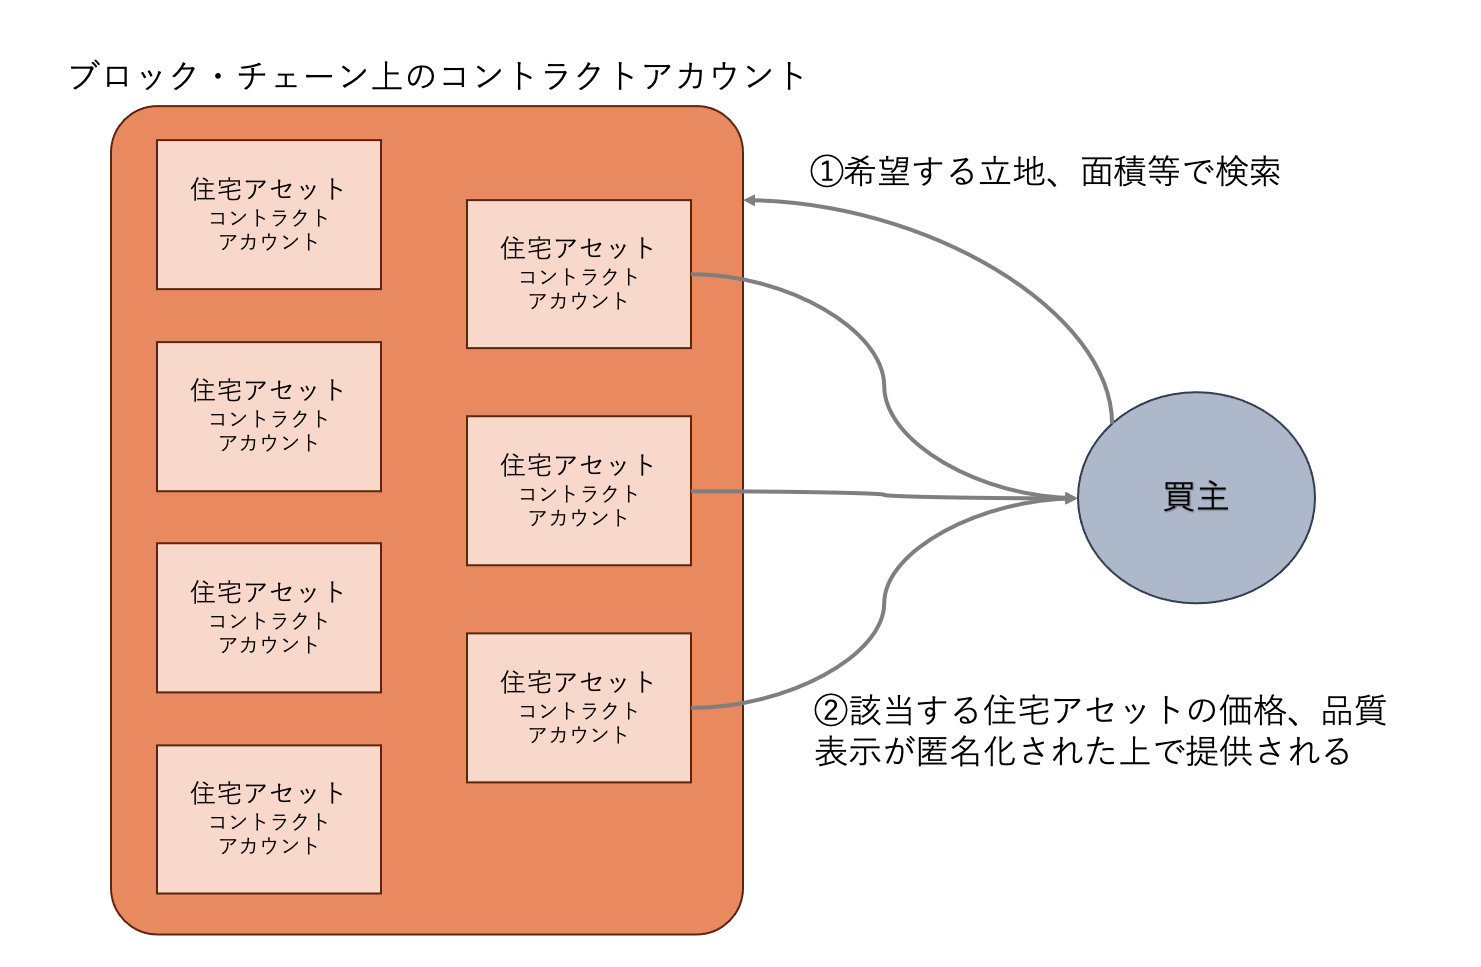
\includegraphics[width=15cm]{search.png}
 \caption{住宅情報の探索}
 \label{search}
\end{figure}

図\ref{spa}は
\begin{figure}
 \centering
 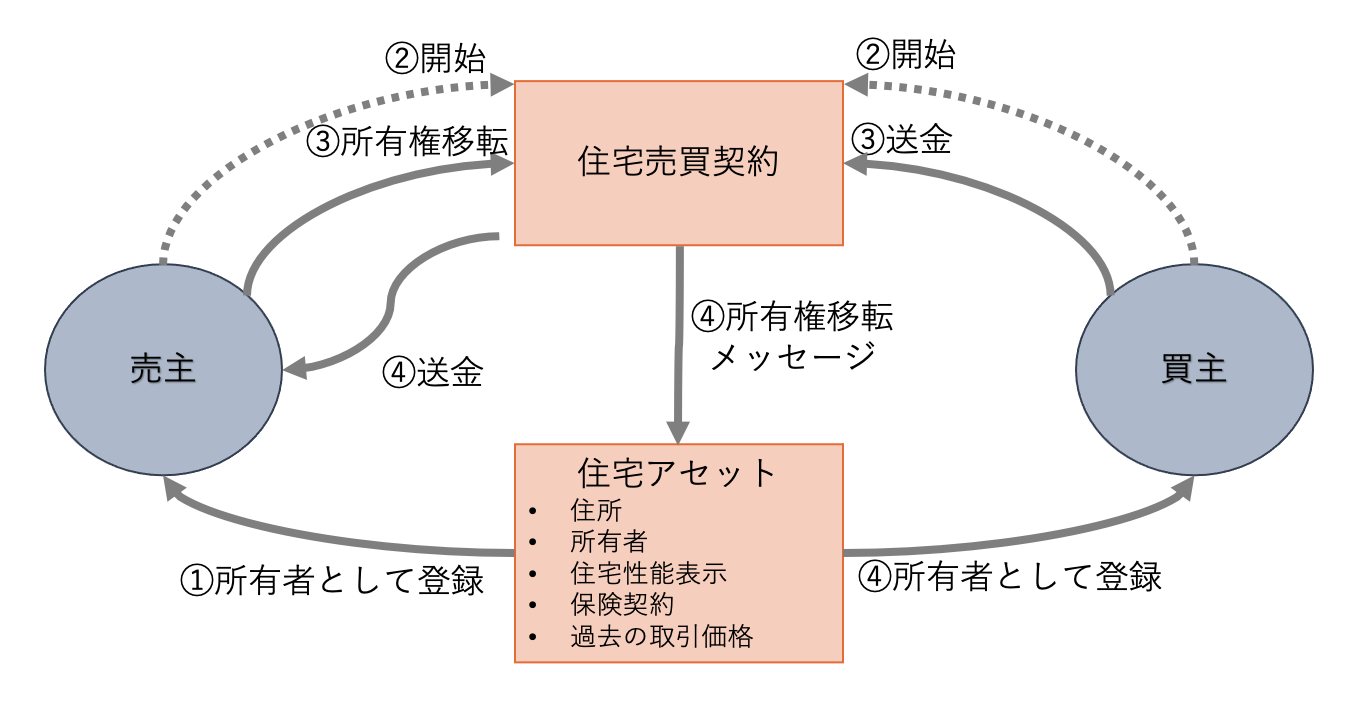
\includegraphics[width=15cm]{spa.png}
 \caption{スマートコントラクトでの売買契約}
 \label{spa}
\end{figure}

図\ref{insurance}は
\begin{figure}
 \centering
 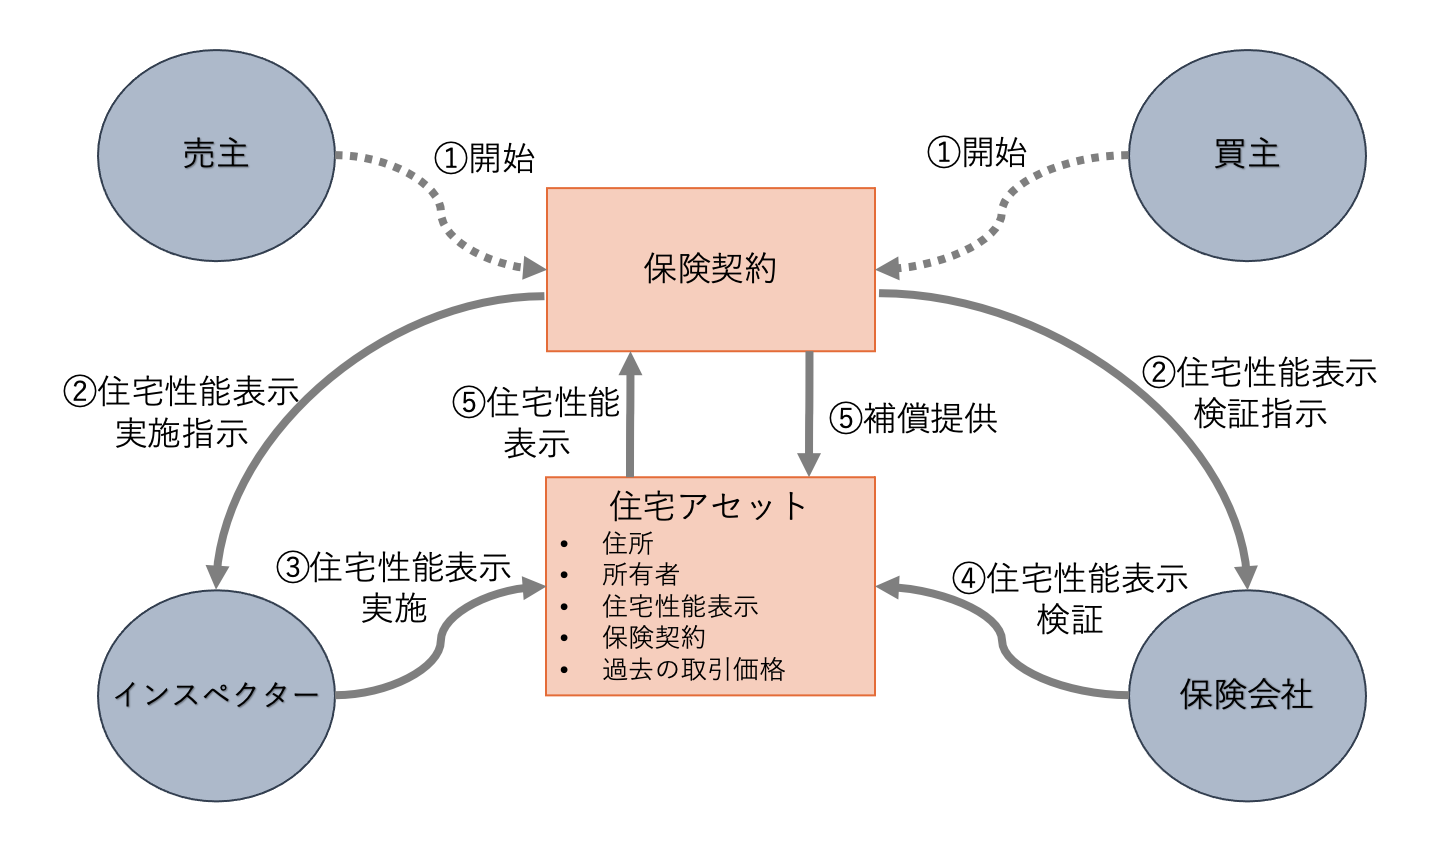
\includegraphics[width=15cm]{insurance.png}
 \caption{保険契約の締結}
 \label{insurance}
\end{figure}

図\ref{flow}は
\begin{figure}
 \centering
 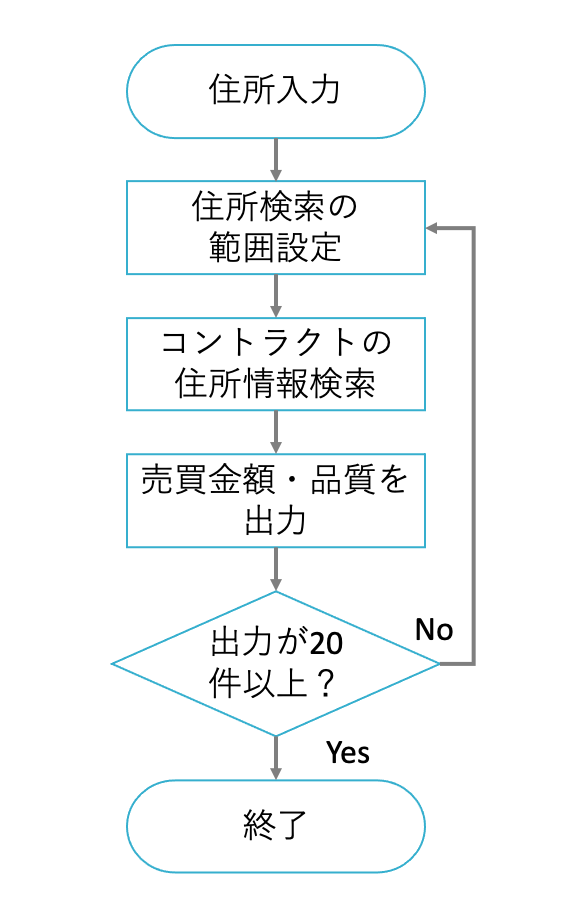
\includegraphics[width=6cm]{flow.png}
 \caption{住宅情報の探索}
 \label{flow}
\end{figure}



\chapter{シミュレーションの実行}
住宅の品質を新築時に決まるものと、所有期間における維持管理によって決まるものに分類し、売主は住宅を売却する段階で品質を変更することはできず、品質を所与として価格設定を行うものとする。売主は住宅を所有するもの中から$\lambda_{d}$の確率で発生するとする。

藤澤(2016)では、売主と買主はそれぞれ同数として、売主、買主の探索の摩擦を考慮していない。しかし、現実の住宅取引においては、売主と買主の数は等しいとは限らない。Duffie(2007)は売主の数が買主よりも少ない場合、取引価格は減少すると指摘している。そこで本研究では、住宅の所有者のうち、一定の確率で住宅を所有する意思が低下し、
\section{住宅取引の関与者}
売主、買主に加えてインスペクター、保険会社%、銀行
が関与すると想定される。これらがそれぞれに外部所有アカウントを持っている。今回検討するモデルでは住宅自体がアカウントをもち、品質情報を持っていることを考える。
\begin{itemize}
	\item 売主
    \par 住宅アセットに所有者として登録されている外部所有アカウント。売買の実施にあたりトランザクションを作成し実行することができる。
    \item 買主
    \par 住宅の取得を希望している外部所有アカウント。Ethereumの場合はEtherを所有している。売買の実施にあたりトランザクションを作成し実行することができる。
    \item インスペクター
    \par 
    \item 保険会社
    %\item 銀行
	\item 住宅アセット	
	\par 土地及び土地に付属する建物の所有権をデジタル資産として表現したコントラクトアカウント。他の住宅アセットと識別するための住所、面積の情報、過去の取引価格、住宅性能表示、保険契約の情報を持っており、これらの情報は第三者から参照可能となっている。
	\item 住宅売買契約
	\item 保険契約

\end{itemize}


\section{ブロックチェーンネットワークの選択}


\section{コントラクト}

\section{匿名化}
Ethereumを基盤としたスマートコントラクトを活用する際の情報の匿名化の手法として、ZK-snaksがある。

zk-SNARKs in Ethereum
Developers have already started integrating zk-SNARKs into Ethereum. What does this look like? Concretely, you can add the building blocks of the verification algorithm to Ethereum in the form of precompiled contracts. Here’s how: run the generator off-chain to produce the proving key and verification key. Any prover can then use the proving key to create a proof, also off-chain. You can then run the general verification algorithm inside a smart contract, using the proof, the verification key, and the public input as input parameters. You can then use the outcome of the verification algorithm to trigger other on-chain activity.
https://consensys.net/blog/blockchain-development/introduction-to-zk-snarks
\section{スマートコントラクトのコスト}
Ethereumブロックチェーンにおいてスマートコントラクトを実行する場合、Gasと呼ばれる手数料が必要となる。コントラクトは通常、実行にあたって使用されるガスの上限であるガスリミットが設定されている。

\section{ゲームのルール}
現在の住宅取引は、売主と買主の間で住宅の品質に関する情報の有無が異なるため、非対称情報ゲームとして記述することができる。売主は所有する住宅の品質を知っており、品質に比べて不当に高い値付けを行うか、品質に応じた値付けを行うかの2つの選択肢をとり得ると想定する。売主は住宅の保有コストを負担しており、住宅の売却ができなかった場合、保有コスト分の損を被る。買主は売主からの価格の提示を受けて買うか買わないか判断し、購入した後で住宅の品質に応じて利得が確定する。住宅の品質を$H$、住宅保有コストを$C_s$、売主が高い値付けをする場合の利鞘を$P$、買主が住宅を購入できない間に負担するコストを$C_b$とすると、売主と買主の各戦略における利得は表\ref{ritoku}となる。

\begin{table}
\begin{center}
\caption{売主・買主の利得}
\label{ritoku}
\begin{tabular}{l|cc}
売主\買主 & 買う & 買わない \\ \hline
高い値付け($H+P$)   &  $P$,  $-P$ &  $-C_s$,  $-C_b$  \\
妥当な値付け($H$)   &  0, 0 &  $-C_s$,  $-C_b$ 
\end{tabular}
\end{center}
\end{table}%


\chapter{評価}


\chapter{関連研究}
Karamitsos et al(2019)\cite{karamitsos2019}は、住宅の賃貸借契約を締結し、賃料の支払いを行い、賃貸借契約終了時の敷金の精算を行うEhtereumブロックチェーンを利用したスマートコントラクトの設計を行なっている。不動産分野におけるスマートコントラクトの活用を論じた論文は数が少なく、比較的早い段階の論文である。スマートコントラクトの概略や設計の考え方に重きが置かれており、現実の不動産分野での利用における課題についてはほとんど触れられていない。不動産分野、住宅分野でのスマートコントラクトの活用は、現実の資産を対象としている事から、スマートコントラクトの対象となる不動産、住宅がどのような特性をもつ資産であるかについてより詳細な検討を行い、その資産の利用者がどのようなニーズを持っているかを検討する必要がある。

\chapter{結論}
本稿では日本の中古住宅の取引におけるスマートコントラクトの活用が、中古住宅の価格や品質の情報を利用可能にする事によって、取引価格の向上や成約率の向上に資することを検証した。日本の家計における住宅資産は、土地の価値も含めると現金・預金等に匹敵する規模があり、その市場価値が減少した場合には家計の投資や消費にマイナスの影響を与える可能性が高い。これまで日本の中古住宅市場は、売主と買主の間で住宅の品質や価格についての情報の非対称性が大きく、レモンの市場となっていた事から活性化していなかった。本稿の検証により、品質情報を含めたスマートコントラクトにより住宅取引を行い、価格情報等の取引情報をブロックチェーン上に公開して情報公開を進めることは、中古住宅取引の活性化に繋がり、中古住宅の取引価格を引き上げると考えられる。スマートコントラクトは、参加者の利便性と情報の信頼性を同時に満たすことのできるアプローチであるが、その活用にあたっては個人情報の取り扱いに配慮する必要がある。加えて、住宅という物的な資産をスマートコントラクトの対象とする場合、住宅の品質情報などを正確にスマートコントラクト上に取り込む仕組みが重要となる。日本では建物状況調査などの取り組みが政策によって推進されていたが、活用が進んでいなかった。これらの仕組みがスマートコントラクトに取り込まれる事によって、信頼性のある資産の情報が全ての参加者に利用可能となる。

本稿では金融機関が住宅取引に与える影響を十分に検証することができなかった。金融機関は住宅ローンの提供により住宅取引に影響を与えている。買主は住宅購入資金を全額自己資金で賄うことは稀であり、住宅ローンを利用することが一般的である。そのため、買主が品質情報や過去の取引情報からある住宅の売出し価格が妥当だと判断しても、金融機関の担保評価が低ければ住宅ローンの融資額が低くなり取引が成立しない。そのため、中古住宅の取引価格が上昇するためには、金融機関の担保評価が上昇することが欠かせない。金融機関の担保評価は、債務者の債務不履行が起きた場合に担保物件の住宅を売却する事により回収できる金額を想定して算出される。中古住宅の品質情報や取引価格の水準情報が参照可能となる事は、金融機関の担保評価においても、担保評価を高めると考えられる。また、本稿のシミュレーションでは、売主と買主の行動に注目し住宅の品質のクラスは単純化した。現実の中古住宅市場は資産の個別性が高く、住宅が所在する立地も異なる事から、一つとして同じ住宅はない。スマートコントラクトが中古住宅市場に与える影響を検討するためには、このような住宅の個別性を踏まえた検証が今後行われる必要がある。


\bibliographystyle{jplain}
\bibliography{export}

\end{document}
